\chapter{Fault  Analysis }
\textit{Probable faults in the system are examined using a  Failure Mode and Effects Analysis (FMEA). In order to decide the importance of handling each fault, the severity and occurrence (SO)  of faults is analyzed. It was decided that the fault analysis is focused on actuators fault detection.}

\label{chap:fault}


\nomenclature[AF]{\textbf{FMEA}}{Failure Mode and Effects Analysis}
\nomenclature[AS]{\textbf{SO}}{Severity and Occurrance}
\nomenclature[AF]{\textbf{FDI}}{Fault Detection and Isolation}
\nomenclature[SF]{$\vec{{F}_{MT}}$}{The fault vector for the magnetorqers}
\nomenclature[SF]{$\vec{{F}_{RW}}$}{The fault vector for the reaction wheels}

A fault in a system can be seen as a sudden shift in the system functionality, however, it might not mean a total shutdown of the system. The faults can be considered as a disturbance in the system, some of which might cause performance loss while others serious deterioration to the system. Failures are distinguished from faults since can cause a total shutdown of the system component. 

In figure \ref{fig:1} a fault tolerant system is shown, which contains an autonomous supervisor that has the ability to switch between various controllers taking into account the type of fault that a component has. The spacecraft block illustrated in the picture is composed of a plant, actuators and sensors and is monitored by the fault detection and isolation (FDI) system, which include detectors that will feed informations to the supervisor in the eventuality of a fault. Based on the information received, the supervisor will establish if a fault occurred or not and in case of a fault the effectors will handle it. Furthermore figure \ref{fig:1} shows the procedure of how faults are handled with various methods. The first step in Fault Analysis is fault modeling which uses a procedure called FMEA.
\begin{figure}[H]
	\begin{minipage}[b]{0.49\linewidth}
		\centering
		\begin{figure}[H]
			\centering
			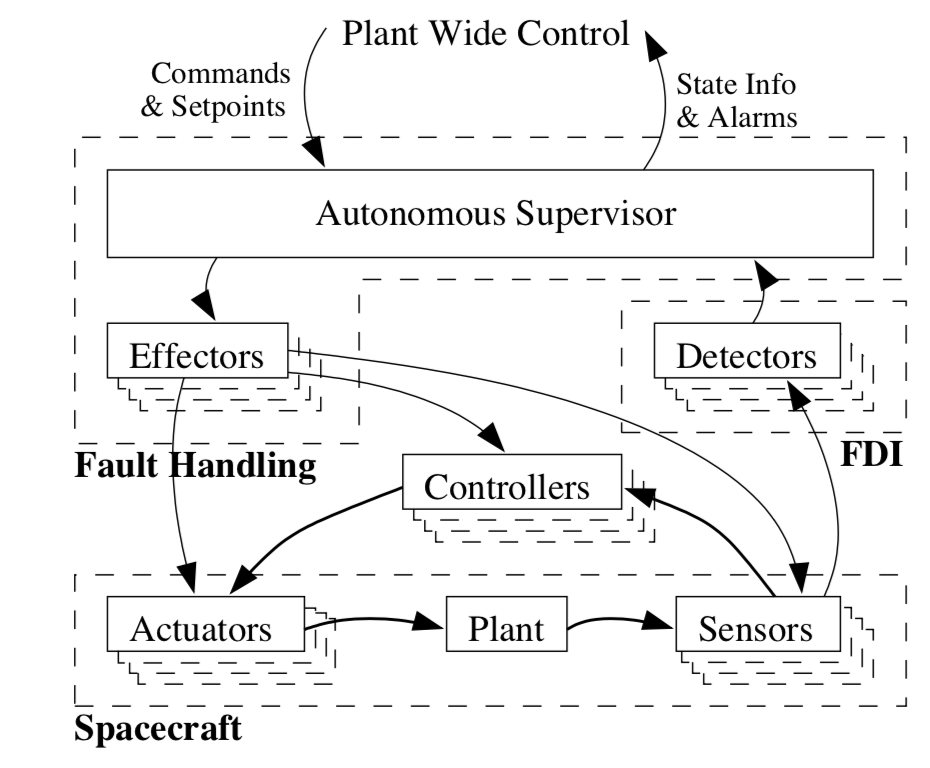
\includegraphics[width=1\linewidth]{figures/FTC}
		\end{figure}
	\end{minipage}\hfill
	\begin{minipage}[b]{0.49\linewidth}
		\centering
		\begin{figure}[H]
			\centering
			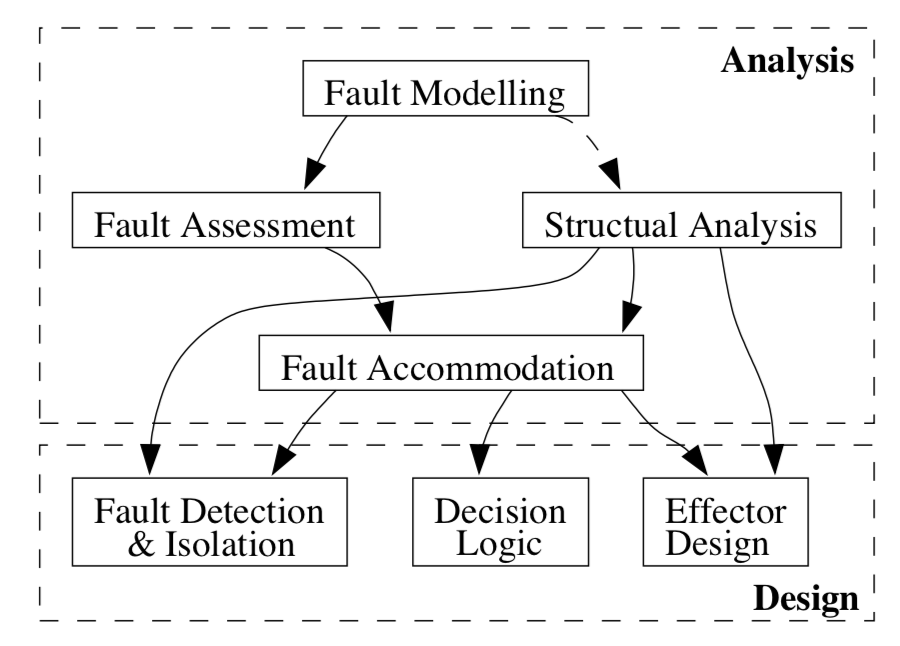
\includegraphics[width=1\linewidth]{figures/FTC_2}
		\end{figure}
	\end{minipage}
			\caption{Fault tolerant system architecture and fault handling using different methods \cite{FTJ}}
				\label{fig:1}
\end{figure}

\section{Failure Mode and Effects Analysis}
A FMEA analysis which is a bottom-up analysis method is performed for the components of the satellite. The main goal of FMEA is to identify possible faults and their effects on components. Another aspect of FMEA analysis is that, the severity of a fault can be determined, offering the opportunity to prioritize the faults by severity and in this way focus on the important faults.

In order to control the attitude of the satellite, two types of actuators are used: magnetorquers and reaction wheels. Potential faults are gathered into tables \ref{tab:mtfault} and \ref{tab:kysymys} describing the effect and cause on the satellite in orbit.

\subsubsection{Magnetorquers}
\begin{table}[H]
	\centering
	\begin{tabular}{|l|l|l|}
		\hline
		\multicolumn{3}{|c|}{\textit{\textbf{Magnetorquers}}}                                          \\ \hline
		\multicolumn{3}{|c|}{Creates a magnetic field that interacts with Earth's magnetic field}                     \\ \hline
		\textbf{Reference} & \textbf{Failure Effect} & \textbf{Failure Cause}                          \\ \hline
		$MT1$                 & Low magnetic field  & \begin{tabular}[c]{@{}l@{}}1) Broken wire or bad soldering\\ 2) Component burned\end{tabular} \\ \hline
		$MT2$                 & Maximum magnetic field power  & Short circuit to the power voltage   \\ \hline
		$MT3$                 & Wrong direction of the magnetic moment & \begin{tabular}[c]{@{}l@{}} 1) Misalignment of the magnetorquer\\ 2) Short circuit between  the \\ magnetorquer and the power voltage \end{tabular} \\ \hline
		$MT4$                 & Wrong  magnetic field magnitude                & Faulty supply voltage                                            \\ \hline
	\end{tabular}
	\caption{Potential faults in the magnetorquers}
	\label{tab:mtfault}
\end{table}
Description of faults in the magnetorquers: 

$\mathcal{F}_{MT1}$: 
The coil might have a broken wire or bad soldering, which can lead to the weakening of the magnetorqer magnetic field. The same effect can arise if an electric component is burned from large currents caused by a fault in the voltage regulator.

$\mathcal{F}_{MT2}$: 
A short circuit in the power supply can lead to maximum magnetic field output.

$\mathcal{F}_{MT3}$:
A misalignment of the magnetorquer  due to transportation or a sudden shift during the launch, could affect the direction of the magnetorquer magnetic field, leading to wrong magnetorquer magnetic moment output.

$\mathcal{F}_{MT4}$:  
A fault supply voltage that could mean lead to uncontrollable magnetorquer magnetic field.

%The fault vector for the magnetorqers is constructed as follows:
%
%$\mathcal {\vec{{F}_{MT}}}$ = [ \ $\mathcal{F}_{MT1}$ \ $\mathcal{F}_{MT2}$ \ $\mathcal{F}_{MT3}$ \ $\mathcal{F}_{MT4}$ ]$^ \mathsf{T}$

\subsubsection{Reaction wheels}
\begin{table}[H]
	\centering
	\begin{tabular}{|l|l|l|}
		\hline
		\multicolumn{3}{|c|}{\textit{\textbf{Reaction wheels}}}                                          \\ \hline
		\multicolumn{3}{|c|}{Produces a torque in order to rotate the satellite}                     \\ \hline
		\textbf{Reference} & \textbf{Failure Effect} & \textbf{Failure Cause}                          \\ \hline
		$RW1$                & Faulty torque orientation & \begin{tabular}[c]{@{}l@{}} Shifting of the flywheel  \\   \end{tabular} \\ \hline
		$RW2$                & Uncontrollable rotation   & A short-circuit in the power supply  \\ \hline
		$RW3$                & Low motor power & Short circuit \\ \hline
		$RW4$                & No torque exerted  &  A fault in windings    \\ \hline
		$RW5$                & Higher power requirement  &  A fault in bearings    \\ \hline
	\end{tabular}
	\caption{Potential faults in the reaction wheels}
	\label{tab:kysymys}
\end{table}
Description of faults in the reaction wheels: 

$\mathcal{F}_{RW1}$: 
A displacement of the flywheel during launch or transportation could result in an error in the controlled torque orientation.

$\mathcal{F}_{RW2}$: 
A short-circuit in the power supply could influence the control of the flywheel by decreasing the range of the control voltage.

$\mathcal{F}_{RW3}$:
A short circuit to the ground due to a broken wire or bad soldering will result in low torque output. 

$\mathcal{F}_{RW4}$:  
Due to a fault in the windings, the flywheel is uncontrollable since the motor can not exert torque.

$\mathcal{F}_{RW5}$:  
If the motor bearings fail, then the motor will need to generate more torque than usual in order to compensate, therefore more power is required.

%The fault vector for the reaction wheels is constructed as follows:
%
%$\mathcal {\vec{{F}_{RW}}}$ = [ \ $\mathcal{F}_{RW1}$ \ $\mathcal{F}_{RW2}$ \ $\mathcal{F}_{RW3}$ \ $\mathcal{F}_{RW4}$ \ $\mathcal{F}_{RW5}$]$^ \mathsf{T}$

In appendix \ref{chap:H} a severity and occurrence evaluation is performed.
%\subsubsection{Fault propagation analysis}
%In order to observe how faults are propagated through the system and the effect of these faults, a FMEA scheme is constructed. Further computation will be on the appendix.
